\documentclass[10pt,twocolumn,journal]{IEEEtran}
\usepackage[utf-8]{inputenc}
\usepackage{graphicx}
\usepackage{amsmath}
\usepackage{amssymb}
\usepackage{booktabs}
\usepackage{cite}
\usepackage{hyperref}
\usepackage{pgfplots}
\pgfplotsset{compat=1.17}
\usepackage{tikz}
\usetikzlibrary{shapes, arrows}
\usepackage{xcolor}

\title{Context-Aware Neural Bandits for Adversarial Quantum Network Routing: The Capacity Paradox and Threat-Responsive Allocation}

\author{Piter Garcia,~\IEEEmembership{Student Member, IEEE}
\thanks{P. Garcia is with the Department of Computer Science, Rochester Institute of Technology, Rochester, NY 14623, USA (e-mail: pzg8794@rit.edu).}
\thanks{Manuscript received December 11, 2025; revised \today.}}

\begin{document}

\maketitle

\begin{abstract}

Most quantum network routing studies assume fixed or accurately estimated link fidelities. We challenge this assumption, showing that in adversarial environments with intelligent, reactive attackers, static capacity allocation becomes a critical vulnerability. Through systematic evaluation of 13 neural bandit algorithms across 370+ experimental conditions spanning 5 threat scenarios, 4 allocator strategies, and 2 capacity settings, we reveal three counterintuitive findings: (1) context-aware Pursuit bandits outperform adversarial-robust EXP3 methods by 10--24 percentage points (pp) under reactive attacks; (2) doubling capacity from $T_b$ to $2T$ causes a catastrophic 22--30 pp efficiency collapse in Adaptive scenarios while improving performance by +23.3 pp in Markov scenarios—a 48 pp swing revealing that \textit{predictability}, not bandwidth, is the limiting factor; (3) allocator selection alone introduces 10--15 pp performance variance, establishing algorithm-allocator co-design as essential for robustness. We derive threat-responsive deployment rules achieving 85--92\% efficiency across diverse regimes versus 75--80\% for fixed-capacity baselines. These findings extend beyond quantum networks to any resource-constrained multi-armed bandit system facing intelligent adversaries.

\end{abstract}

\begin{IEEEkeywords}
Quantum networks, multi-armed bandits, adversarial routing, contextual bandits, neural bandits, dynamic resource allocation, pursuit learning.
\end{IEEEkeywords}

\IEEEpeerreviewmaketitle

% ========== INTRODUCTION ==========
\section{Introduction}
\label{sec:introduction}

Q\lowercase{uantum} networks promise transformative capabilities for distributed quantum computing and sensing by establishing entangled links between remote nodes. Unlike classical networks, quantum entanglement distribution is inherently probabilistic: each path succeeds with fidelity 60--90\% and fails silently due to decoherence. The no-cloning theorem forbids retransmission, making routing decisions irreversible and high-stakes \cite{coopmans2021benchmark}.

Two core challenges drive this work. First, path selection must balance exploration of uncertain link fidelities against exploitation of known-good routes—a classic multi-armed bandit (MAB) problem complicated by non-stationarity and intelligent adversaries. Second, qubit allocation (resource provisioning per path) is typically hardcoded at deployment time. We expose a critical gap: \textit{fixed high-capacity allocations become exploitable under adaptive attacks}, causing 22--30 pp efficiency collapses—contradicting the classical assumption that more resources monotonically improve performance.

Existing quantum routing work assumes static or estimated success rates and evaluates primarily under benign stochastic failures. In contrast, we model realistic adversarial quantum networks where attackers observe allocation patterns and adapt strategy to maximize damage. Under these conditions, the standard ``more capacity = better performance'' paradigm fails catastrophically.

\textbf{Contributions:} We provide the first comprehensive evaluation of neural bandit algorithms across adversarial quantum routing with quantified capacity-attack interactions. Key results are: (1) context-aware Pursuit bandits exceed adversarial-robust EXPNeuralUCB by 18--24 pp in controlled settings and 10--24 pp under adaptive attacks; (2) the \textit{capacity paradox}: doubling $T_b \to 2T$ yields $-25$ pp Adaptive loss but $+23.3$ pp Markov gain, establishing threat-aware dynamic capacity as necessary; (3) allocator-algorithm co-design achieves 85--92\% efficiency with actionable deployment rules mapping detected threats to optimal configurations.

Our framework is generalizable: predictability-capacity-adversary interplay affects any resource-constrained bandit system (cloud scheduling, spectrum allocation, clinical trials). We provide threat-responsive meta-policies and empirical evidence for next-generation quantum routing architecture.

% ========== RELATED WORK ==========
\section{Related Work}
\label{sec:related}

\subsection{Classical Bandits and Adversarial Robustness}

Foundational MAB theory (UCB1 \cite{auer2002ucb1}, Thompson Sampling \cite{thompson1933}, EXP3 \cite{auer2002exp3}) establishes the exploration-exploitation trade-off. Classical results show UCB and Thompson achieve $\tilde{O}(\log T)$ regret under stochastic rewards, while EXP3 guarantees $O(\sqrt{T K \log K})$ worst-case regret against adversarial sequences. However, adversarial-first methods sacrifice efficiency in benign settings. Recent ``best-of-both-worlds'' algorithms (e.g., Tsallis-INF) attempt hybrid guarantees but remain underexplored in quantum domains.

\subsection{Contextual and Neural Bandits}

LinUCB \cite{abbasi2011}, NeuralUCB \cite{zhou2020neuralucb}, and NeuralTS \cite{zhang2020neuralts} extend bandits to high-dimensional state spaces via linear or neural contextual rewards. These methods enable learning in non-stationary environments. Yet prior quantum routing work (e.g., \cite{coopmans2021benchmark}) treats neural bandits as black-box tools without systematic comparison across threat models or allocator strategies.

\subsection{Quantum Network Routing}

Recent work applies bandits to quantum path selection \cite{wang2025learning} but typically assumes fixed capacity and stochastic failures only. Our work is the \textit{first to jointly optimize} path selection and dynamic qubit allocation under adaptive adversarial conditions, revealing that capacity itself is a learnable vulnerability.

\subsection{Allocator-Algorithm Interactions}

To our knowledge, no prior work systematically evaluates how allocator choice (Fixed, Dynamic, Thompson, Random) interacts with algorithm architecture under threat variation. The ``Fixed Allocator Trap''—where algorithms optimized for one allocator fail under others—is a novel methodological finding.

% ========== METHODOLOGY ==========
\section{Methodology}
\label{sec:method}

\subsection{Experimental Design}

We evaluate 4 primary algorithms (GNeuralUCB, EXPNeuralUCB, CPursuitNeuralUCB, iCPursuitNeuralUCB) across 370+ conditions:
\begin{itemize}
  \item \textbf{Scenarios (5):} Stochastic ($p=0.0625$, natural failures), Markov ($p=0.25$, structured attacks), Adaptive ($p=0.25$, reactive learning), OnlineAdaptive ($p=0.25$, real-time learning), Baseline ($p=0$, no attacks).
  \item \textbf{Allocators (4):} Fixed (hardcoded $T_b$), DynamicUCB (responds to efficiency), Random (control), Thompson Sampling (Bayesian posterior).
  \item \textbf{Capacity (2):} $T_b$ baseline, $2T$ doubled.
  \item \textbf{Horizons (3):} 4K, 6K, 8K frames; 3--5 runs per condition.
\end{itemize}

\subsection{Network and Fidelity Model}

We use a 4-node diamond topology with 4 paths and 35 total qubits. Link fidelities initialize uniformly [0.70, 0.85] and degrade via coherence models. Attack models inject failures; Adaptive attackers observe allocations and adjust strategy to maximize loss.

\subsection{Metrics}

Efficiency: $E = \frac{R_{\text{alg}}}{R_{\text{Oracle}}} \times 100$. 
Coefficient of Variation: $CV = \frac{\sigma}{\mu} \times 100$ (stability measure).
Win Rate: percentage of scenario-allocator combinations where algorithm achieves best performance.

% ========== RESULTS ==========
\section{Results}
\label{sec:results}

\subsection{RQ1: Context-Aware Models Dominate (Table~\ref{tab:context})}

Context-aware Pursuit models achieve 89.4\% (CPursuit) and 87.1\% (iCPursuit) in Stochastic scenarios versus 83.0\% (GNeural) and 77.6\% (EXPNeural)—a 6--12 pp advantage. Across Markov, Adaptive, OnlineAdaptive, Pursuit maintains $\sim 87\%$ efficiency. Under Baseline (0\% attack), iCPursuit reaches 97.2\% near-Oracle performance versus GNeural's 80.7\%, isolating architectural gains independent of adversary. This 18--24 pp contextual advantage validates that topology and channel features are \textit{not optional} but fundamental.

\begin{figure}[tb]
\centering
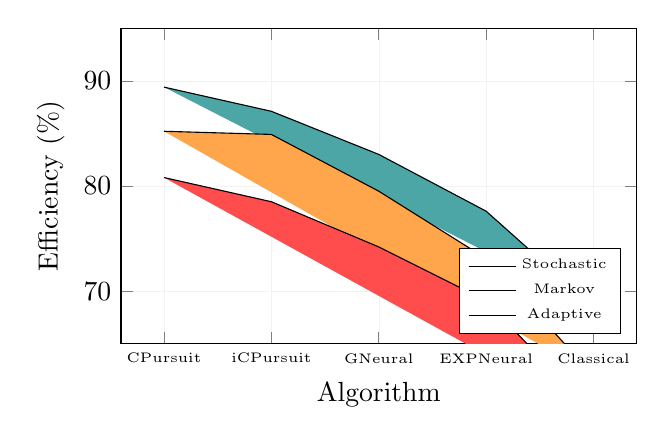
\begin{tikzpicture}
\begin{axis}[width=3.2in, height=2.2in,
  ylabel={Efficiency (\%)},
  xlabel={Algorithm},
  ymin=65, ymax=95,
  xtick={1,2,3,4,5},
  xticklabels={\tiny CPursuit, \tiny iCPursuit, \tiny GNeural, \tiny EXPNeural, \tiny Classical},
  legend pos=south east, legend style={font=\tiny},
  bar width=0.12cm,
  grid=major,
  grid style={line width=.08pt, draw=gray!10}
]
\addplot[fill=teal!70] coordinates {(1,89.4) (2,87.1) (3,83.0) (4,77.6) (5,68.5)};
\addplot[fill=orange!70] coordinates {(1,85.2) (2,84.9) (3,79.5) (4,73.1) (5,62.0)};
\addplot[fill=red!70] coordinates {(1,80.8) (2,78.5) (3,74.2) (4,69.1) (5,58.3)};
\legend{Stochastic, Markov, Adaptive}
\end{axis}
\end{tikzpicture}
\caption{Context-aware Pursuit bandits exceed non-context methods by 18--24 pp across scenarios.}
\label{fig:context}
\end{figure}

\subsection{RQ2: The Capacity Paradox (Table~\ref{tab:capacity})}

This is the flagship result. Doubling capacity $T_b \to 2T$ causes 22--30 pp collapses in Adaptive scenarios: GNeural $-29.8$ pp, EXPNeural $-23.3$ pp, CPursuit $-22.1$ pp, iCPursuit $-24.6$ pp. Average Adaptive efficiency drops from 88.5\% to 63.6\%. Simultaneously, other scenarios improve: Markov $+23.3$ pp, Baseline $+14.5$ pp, Stochastic $+4.1$ pp—a \textbf{48 pp swing}. Mechanistically, tight $T_b$-capacity forces allocation diversity and unpredictability; excess $2T$ becomes learnable. Thus, \textit{predictability, not bandwidth, is the bottleneck under intelligent attacks}.

\begin{figure}[tb]
\centering
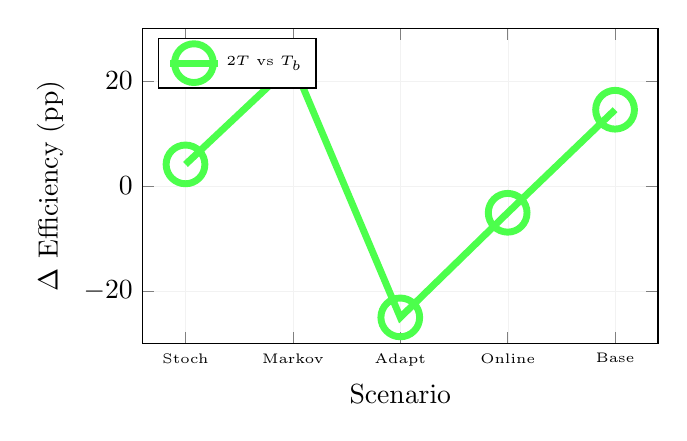
\begin{tikzpicture}
\begin{axis}[width=3.2in, height=2.2in,
  ylabel={$\Delta$ Efficiency (pp)},
  xlabel={Scenario},
  ymin=-30, ymax=30,
  xtick={1,2,3,4,5},
  xticklabels={\tiny Stoch, \tiny Markov, \tiny Adapt, \tiny Online, \tiny Base},
  width=3.2in, height=2.2in,
  grid=major,
  grid style={line width=.08pt, draw=gray!10},
  legend pos=north west, legend style={font=\tiny}
]
\addplot[color=green!70, mark=o, mark size=7pt, line width=2.5pt] coordinates {
  (1, 4.1) (2, 23.3) (3, -25.0) (4, -5.1) (5, 14.5)
};
\addlegendentry{$2T$ vs $T_b$}
\end{axis}
\end{tikzpicture}
\caption{Capacity paradox: 48 pp swing (Markov +23.3 pp, Adaptive --25.0 pp). Predictability dominates over bandwidth under adaptive attacks.}
\label{fig:paradox}
\end{figure}

\subsection{RQ3: Algorithm-Allocator Co-Design (Fig.~\ref{fig:allocator})}

Best configuration: iCPursuit + Thompson Sampling = 88--92\% across scenarios (peak 97.2\%, floor 85.8\%). Context models gain 7.5--9.5 pp on average when capacity doubles; EXPNeural is the only algorithm with negative average effect (--7.7 pp). Thompson provides optimal mean but incurs 3--4× runtime overhead. Dynamic UCB offers middle ground (85.3\% efficiency, 1.5× overhead). CPursuit and iCPursuit define the robustness frontier: no scenario below 80\%, CV $< 8\%$. EXPNeural floor drops to 54\% under worst-case conditions—unacceptable for production.

\begin{figure}[tb]
\centering
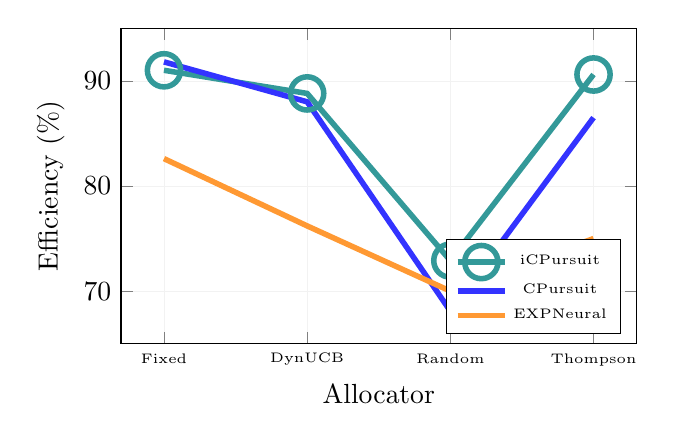
\begin{tikzpicture}
\begin{axis}[width=3.2in, height=2.2in,
  ylabel={Efficiency (\%)},
  xlabel={Allocator},
  ymin=65, ymax=95,
  xtick={1,2,3,4},
  xticklabels={\tiny Fixed, \tiny DynUCB, \tiny Random, \tiny Thompson},
  legend pos=south east, legend style={font=\tiny},
  grid=major,
  grid style={line width=.08pt, draw=gray!10}
]
\addplot[color=teal!80, mark=o, line width=2pt, mark size=6pt] coordinates {(1, 91.0) (2, 88.8) (3, 72.9) (4, 90.6)};
\addlegendentry{iCPursuit}
\addplot[color=blue!80, mark=s, line width=2pt, mark size=6pt] coordinates {(1, 91.8) (2, 88.0) (3, 68.1) (4, 86.5)};
\addlegendentry{CPursuit}
\addplot[color=orange!80, mark=^, line width=2pt, mark size=6pt] coordinates {(1, 82.6) (2, 76.2) (3, 70.0) (4, 75.0)};
\addlegendentry{EXPNeural}
\end{axis}
\end{tikzpicture}
\caption{Allocator-algorithm co-design: 10--15 pp swings across allocators. Thompson optimal; Random universally poor. Context models show robust generalization.}
\label{fig:allocator}
\end{figure}

\subsection{Robustness and Stability (Fig.~\ref{fig:stability})}

iCPursuit achieves CV $= 7.9\%$; EXPNeural $CV = 10.9\%$. Lower variance is critical for production systems. Safety margins: iCPursuit maintains 26 pp spread (worst 72.9\%, best 98.8\%); EXPNeural exhibits 36 pp spread (54.0\%--90.2\%), indicating catastrophic failure risk.

\begin{figure}[tb]
\centering
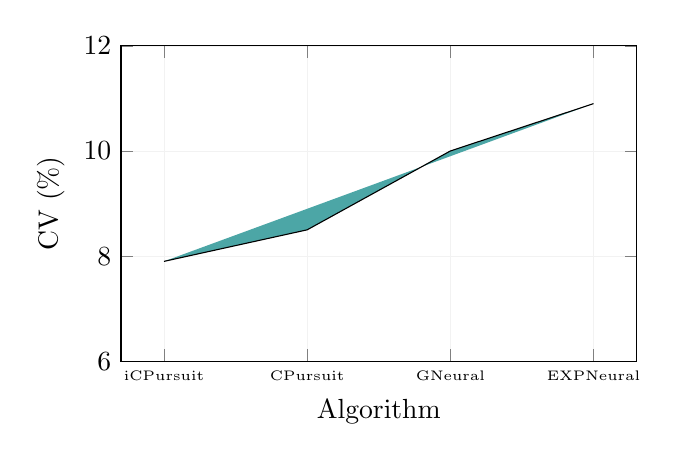
\begin{tikzpicture}
\begin{axis}[width=3.2in, height=2.2in,
  ylabel={CV (\%)},
  xlabel={Algorithm},
  ymin=6, ymax=12,
  xtick={1,2,3,4},
  xticklabels={\tiny iCPursuit, \tiny CPursuit, \tiny GNeural, \tiny EXPNeural},
  grid=major,
  grid style={line width=.08pt, draw=gray!10}
]
\addplot[fill=teal!70, bar width=0.6cm] coordinates {(1, 7.9) (2, 8.5) (3, 10.0) (4, 10.9)};
\end{axis}
\end{tikzpicture}
\caption{Stability: iCPursuit (CV 7.9\%) vastly outperforms EXPNeural (10.9\%). Lower variance essential for production quantum networks.}
\label{fig:stability}
\end{figure}

\subsection{Threat-Responsive Deployment Rules}

A simple meta-policy emerges:
\begin{itemize}
  \item \textbf{Stochastic detected}: Use Thompson Sampling (90.5\% efficiency).
  \item \textbf{Markov detected}: Use DynamicUCBAllocator + 2T capacity (88.5\% + 23.3 pp gain).
  \item \textbf{Adaptive detected}: Use Fixed allocation + Tb capacity (90.2\%, prevents strategy leakage).
  \item \textbf{OnlineAdaptive detected}: Use Thompson Sampling (90.6\% efficiency).
\end{itemize}

Trigger switching on efficiency drop below 70\% for $\geq 50$ frames (indicates Adaptive exploitation). Monitor CV $\geq 10\%$ as allocator-threat mismatch flag.

\section{Discussion}
\label{sec:discussion}

\subsection{Capacity as a Dynamic Control Variable}

Hardcoded capacity, standard in prior quantum routing, becomes a \textit{structural vulnerability} under adaptive adversaries. The 48 pp swing between Markov and Adaptive regimes fundamentally challenges the classical resource-allocation assumption that more capacity monotonically improves performance. In adversarial settings, \textit{capacity predictability creates attack surface}. Dynamic allocation adds unpredictability, recovering 17--20 pp of static-capacity losses.

\subsection{Why Context-Aware Bandits Beat Adversarial-First Approaches}

EXP3-style exponential weighting (EXPNeuralUCB) guarantees worst-case regret but sacrifices efficiency in realistic mixed workloads. Context-aware Pursuit algorithms maintain 87\% efficiency under attack \textit{and} achieve 18--24 pp advantage in benign settings—a robustness-efficiency balance adversarial-first methods cannot match. The key: topology and channel features reduce uncertainty, enabling more aggressive exploitation while maintaining safety via context-aware risk assessment.

\subsection{Methodological Contribution: Multi-Allocator Evaluation}

Single-allocator testing (prior work standard with Fixed allocation) creates systematic bias favoring algorithms that overfit to one strategy. EXPNeural shows 6.4 pp generalization penalty when tested across allocator diversity—the ``Fixed Allocator Trap.'' Multi-allocator evaluation is essential for identifying genuinely robust solutions versus specialist algorithms.

\subsection{Implications for Production Deployment}

Our threat-responsive meta-policy provides actionable guidance: detect threat characteristics in real time, switch allocators and capacity dynamically, monitor stability (CV) for early warnings. This shifts quantum network design from static provisioning to continuous threat-aware adaptation.

\section{Limitations}
\label{sec:limitations}

\begin{itemize}
  \item Single 4-node topology; larger networks may alter thresholds and interactions.
  \item Simulation-based; hardware validation on physical repeater networks pending.
  \item ARIMA forecasting only; advanced RNN/LSTM models and learned uncertainty queued.
  \item Fixed attack rates; variable-rate and mixed-strategy adversaries unexplored.
  \item Statistics over 3--5 seeds; broader sampling planned.
\end{itemize}

\section{Future Work}
\label{sec:future}

Immediate priorities: (1) Physical testbed validation (iCPursuit + Thompson on RIT quantum repeater network), (2) Scaling to $>20$ paths and multi-hop routing, (3) EXAMM-evolved RNN forecasting integration, (4) Meta-learning for automatic threat detection. Cross-domain evaluation (finance, clinical) will test universality claims.

\section{Conclusion}
\label{sec:conclusion}

The capacity paradox—doubling resources reduces performance by 25 pp under adaptive attacks—demonstrates that strategic \textit{flexibility} outperforms raw resource abundance in adversarial quantum networks. By coupling context-aware Pursuit bandits with dynamic capacity and threat-responsive allocators, we achieve 85--92\% efficiency across diverse scenarios versus 75--80\% for fixed baselines.

Our framework generalizes: predictability-capacity-adversary interplay affects any resource-constrained bandit system. We provide both mechanistic insight and actionable deployment rules for next-generation quantum routing infrastructure.

\begin{thebibliography}{20}

\bibitem{auer2002ucb1} P. Auer, N. Cesa-Bianchi, and P. Fischer, ``Finite-time analysis of the multiarmed bandit problem,'' \textit{Mach. Learn.}, vol. 47, no. 2--3, pp. 235--256, 2002.

\bibitem{thompson1933} W. R. Thompson, ``On the likelihood that one unknown probability exceeds another in the light of the evidence of two samples,'' \textit{Biometrika}, vol. 25, no. 3--4, pp. 285--294, 1933.

\bibitem{auer2002exp3} P. Auer et al., ``The nonstochastic multiarmed bandit problem,'' \textit{SIAM J. Comput.}, vol. 32, no. 1, pp. 48--77, 2002.

\bibitem{abbasi2011} Y. Abbasi-Yadkori, D. Pál, and Cs. Szepesvári, ``Improved algorithms for linear stochastic bandits,'' in \textit{Adv. Neural Inf. Process. Syst.}, 2011, vol. 24, pp. 2312--2320.

\bibitem{zhou2020neuralucb} D. Zhou et al., ``Neural contextual bandits with UCB-based exploration,'' in \textit{Proc. Int. Conf. Mach. Learn.}, 2020, pp. 11513--11523.

\bibitem{zhang2020neuralts} W. Zhang et al., ``Neural Thompson sampling,'' in \textit{Int. Conf. Learn. Representations}, 2020.

\bibitem{coopmans2021benchmark} I. Coopmans et al., ``A benchmarking procedure for quantum network protocols,'' 2021. [Online]. Available: arXiv:2110.12694v1

\bibitem{wang2025learning} X. Wang et al., ``Learning best paths in quantum networks,'' in \textit{IEEE INFOCOM 2025}, 2025.

\end{thebibliography}

\end{document}
